%-------------------------------------------------
\subsection{Essential Background II}
\subsubsection{Expectation Algebra}
\begin{frame}{The Background Break - Expectation Algebra}
    % \begin{columns}
        % \column{0.5\textwidth}
        The necessary mathematical background for Kalman Filter:
            \begin{itemize}
                \item Matrix Operations: Vector/matrix addition and multiplication, transpose, Matrix inverse, Symmetric matrices
                \item Expectation Algebra
                \item Multivariate Normal Distribution (Covariance and Covariance Matrices)
            \end{itemize}
        \textbf{Expectation Algebra}
        \begin{itemize}
            \item The expectation of a random variable $X$ equal the mean of $X$: $E(X)=\mu_X$.
        \end{itemize}
         \begin{table}[]
            \centering
            \begin{tabular}{ll}
                \toprule
                \textbf{Rule} & \textbf{Notes} \\
                \toprule
                $E(X) = \mu_X = \sum x p(x)$ & $p(x)$ is PDF of $x$ \\
                $E(a) = a$ & $a$ is constant\\
                $E(aX) = aE(x)$ & $--$\\
                $E(a\pm X) = a\pm E(x)$ & $--$\\
                $E(a\pm bX) = a\pm bE(x)$ & $b$ is constant\\
                $E(X\pm Y) = E(x) \pm E(Y)$ & $Y$ is another R.V.\\
                $E(XY) = E(X)E(Y)$ & $X, Y$ are independent\\
                \bottomrule
            \end{tabular}
            \caption{Expectation Rules}
            \label{tab:ExpectationRules}
        \end{table}
        % \column{0.5\textwidth}
    % \end{columns}
\end{frame}

%-------------------------------------------------

\begin{frame}{The Background Break - Expectation Algebra}
    % \begin{columns}
        % \column{0.5\textwidth}
        The following table includes the variance and covariance expectation rules.
        \begin{itemize}
            \item Variance of a R.V. $X$: $V(X) = E\left((X-\mu_X)^2\right)$
            \item Covariance of R.V. $X$ and $Y$: $COV(X,Y) = E\left((X-\mu_X)(Y-\mu_Y)\right)$
        \end{itemize}
         \begin{table}[]
            \centering
            \begin{tabular}{ll}
                \toprule
                \textbf{Rule} & \textbf{Notes} \\
                \toprule
                $V(a) = 0$ & Variance of a constant $a$\\[0.7em]
                $V(a\pm X) = V(X)$ & Variance of $X$\\[0.7em]
                $V(X) = E(X^2) - \mu_X^2$ & $--$\\[0.7em]
                $V(a\pm X) = a^2 V(X)$ & $a$ is constant\\[0.7em]
                $COV(X,Y) =E(XY) + \mu_X \mu_Y$ & Covariance of $X$ and $Y$\\[0.7em]
                $COV(X,Y) = 0$ & If $X$ and $Y$ are Independent\\[0.7em]
                $V(X\pm Y) = V(X) + V(Y) \pm 2COV(X,Y)$ & \\[0.7em]
                $V(XY) \neq V(X) V(Y)$ & \\[0.7em]
                \bottomrule
            \end{tabular}
            \caption{Variance and Covariance Expectation Rules}
            \label{tab:Var_CoVar_Rules}
        \end{table}
\end{frame}

%-------------------------------------------------
\begin{frame}{The Background Break - Multivariate Normal Distribution}
\begin{itemize}
\item Introduction to the Kalman Filter: 
    \begin{itemize}
        \item The Kalman Filter output is a random variable.
        \item The mean of the random variable is the state estimate.
        \item The variance represents the estimation uncertainty.
        \item It provides us with the estimate and the level of confidence of its estimate.
    \end{itemize}
\item One-dimensional Kalman Filter equations include four uncertainty variables:
    \begin{enumerate}
        \item \(p_{n,n}\) is the variance of an estimate (the current state).
        \item \(p_{n+1,n}\) is the variance of a prediction (the next state).
        \item \(r_n\) is the measurement variance.
        \item \(q\) is the process noise.
    \end{enumerate}

\item Multivariate Kalman Filter
    \begin{itemize}
        \item Describes the system state by a vector with more than one variable.
        \item For example, object’s position on the plane: \[x = \begin{bmatrix} x \\ y \end{bmatrix}\] 
        \item The Kalman Filter output is a multivariate random variable.
        \item A covariance matrix describes the squared uncertainty of the multivariate random variable.
    \end{itemize}

\item Uncertainty variables of multivariate Kalman Filter
    \begin{itemize}
        \item The uncertainty variables are represented by covariance matrices:
        \begin{enumerate}
            \item \(P_{n,n}\) describes the squared uncertainty of an estimate.
            \item \(P_{n+1,n}\) describes the squared uncertainty of a prediction.
            \item \(R_n\) describes the squared measurement uncertainty.
            \item \(Q\) describes the process noise.
        \end{enumerate}
    \end{itemize}
\end{itemize}    
\end{frame}
%-------------------------------------------------
\subsubsection{Covariance}
\begin{frame}{The Background Break - Multivariate Normal Distribution}
    \begin{itemize}
        \item Covariance is a measure of the strength of the correlation between two or more sets of random variates.
        \item On the x-y plane, variance in measurements exists due to random error.
    \end{itemize}
        \begin{itemize}
            \item \textbf{Uncorrelated measurements:}
            \begin{itemize}
                \item The x and y values don't depend on each other. The covariance of x and y equals zero.
                \item For the blue data set, a circular distribution shape indicates equal variance.
                \item For the red data set, an elliptic distribution shape indicates greater variance in x values.
            \end{itemize}
            \item \textbf{Correlated measurements:}
            \begin{itemize}
                \item Dependency exists between x and y values.
                \item For the green data set, positive correlation and covariance due to concurrent increase.
                \item For the cyan data set, negative correlation and covariance due to inverse changes.
            \end{itemize}
        \end{itemize}
    \begin{figure}
        \centering
    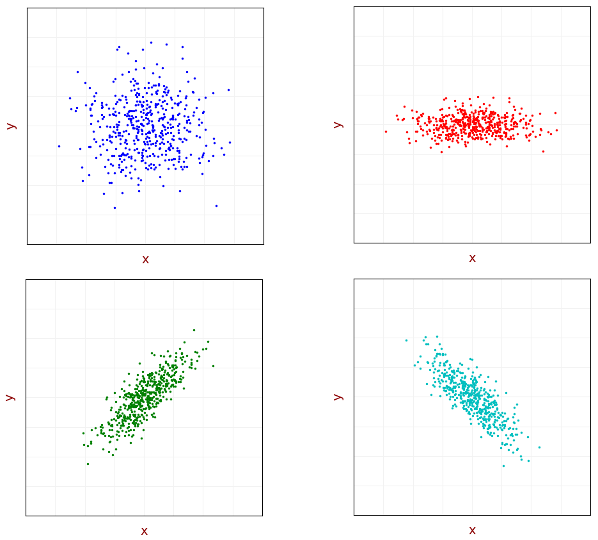
\includegraphics[width=0.4\textwidth]{Figures/Background2/CovarianceIllustration.png}
        \caption{Examples of different measurement sets.}
    \end{figure}

\end{frame}
%--------------------------------------------------------------------
\begin{frame}{The Background Break - Covariance}
The covariance between population $X$ and population $Y$ with size $N$
    \begin{align}
       \text{COV} (X, Y) & = \frac{1}{N} \sum_{i=1}^{N} (x_i - \mu_x)(y_i - \mu_y)\nonumber\\ & = \frac{1}{N} \sum_{i=1}^{N} (x_i y_i) - \mu_x \mu_y \nonumber
    \end{align}
The covariance of a sample with size $N$ is normalized by $N - 1$
    \begin{align}
     \text{COV} (X, Y) & = \frac{1}{N - 1} \sum_{i=1}^{N} (x_i - \mu_x)(y_i - \mu_y)\nonumber \\ &= \frac{1}{N - 1} \left( \sum_{i=1}^{N} x_i y_i \right) - \frac{N}{N - 1} \mu_x \mu_y \nonumber\\
     & = \frac{1}{N - 1}{\mathbf{x}^T y - \frac{N}{N - 1} \mu_x \mu_y}\nonumber \quad [\text{In vector notation}]\\
     & = \frac{1}{N - 1}\mathbf{x}^T y \quad [\text{For a zero-mean random variable}]\nonumber
     \end{align}
\end{frame}

%-------------------------------------------------
\subsubsection{Covariance Matrix}
\begin{frame}{The Background Break - Covariance Matrix}
A covariance matrix is a square matrix that represents the covariance between each
pair of elements in a given multivariate random variable.

For a two-dimensional random variable, the covariance matrix is given by
\begin{equation*}
    \Sigma = 
    \begin{bmatrix}
        \sigma_{xx} & \sigma_{xy} \\
        \sigma_{yx} & \sigma_{yy}
    \end{bmatrix}
    =
    \begin{bmatrix}
        \sigma^2_{x} & \sigma_{xy} \\
        \sigma_{yx} & \sigma^2_{y}
    \end{bmatrix}
    =
    \begin{bmatrix}
        \text{VAR}(x) & \text{COV}(x, y) \\
        \text{COV}(y, x) & \text{VAR}(y)
    \end{bmatrix}
\end{equation*}
Note that the off-diagonal entries of the covariance matrix are equal since $\text{COV}(x, y) =
\text{COV}(y, x)$. If $x$ and $y$ are uncorrelated, the off-diagonal entries of the covariance
matrix are zero.


\textbf{Properties of the covariance matrix:}
\begin{itemize}
    \item The diagonal entries of this covariance matrix are the variances of the components of the multivariate random variable:
    $$\Sigma_{ii} = \sigma^2_{i}$$
    \item Since the diagonal entries are all non-negative, the trace (the sum of diagonal entries) of this covariance matrix is non-negative:
    $$\text{tr}(\mathbf{\Sigma}) = \sum_{i=1}^{n} \Sigma_{ii} \geq 0$$ 
    \item Since \(\Sigma_{ij} = \sigma_{ij} = \sigma_{ji} = \Sigma_{ji}\), the covariance matrix is symmetric:
    $$\mathbf{\Sigma} = \mathbf{\Sigma^T}$$
    \item The covariance matrix is \textbf{positive semidefinite}. The matrix \(\mathbf{A}\) is called positive semidefinite if \(\mathbf{v}^T \mathbf{A} \mathbf{v} \geq 0\), for any vector \(v\). \textbf{The eigenvalues of \(\mathbf{A}\) are non-negative}.
\end{itemize}

\end{frame}
%-------------------------------------------------
\subsubsection{Covariance Matrix and Expectation}
\begin{frame}{The Background Break - Expectation Algebra - Covariance Matrix and Expectation}
\begin{itemize}
    \item Assume a vector $\mathbf{x}$ with $k$ elements:
        \begin{equation*}
            \centering
            \mathbf{x}=\begin{bmatrix}
            x_1\\
            x_2\\
            \vdots\\
            x_k\\
            \end{bmatrix}
            \end{equation*}
    \item The covariance matrix of the vector $\mathbf{x}$ is:
            \begin{align*}
            \centering
            COV(\mathbf{x}) = & E\left((\mathbf{x} -\mathbf{\mu}_x)(\mathbf{x} -\mathbf{\mu}_x)^T\right)\\
            = & E\left(\begin{bmatrix}
            (x_1-\mu_{x_1})\\
            (x_2-\mu_{x_2})\\
            \vdots\\
            (x_k-\mu_{x_k})\\
            \end{bmatrix}
            \Big[(x_1-\mu_{x_1})~~(x_2-\mu_{x_2})~~\cdots~~ (x_k-\mu_{x_k})\Big]
            \right)
            \end{align*}
\end{itemize}
\end{frame}


%-------------------------------------------------------
\subsubsection{Multivariate Normal Distribution}
\begin{frame}{The Background Break - Multivariate Normal Distribution}

Univariate Gaussian distribution:
$$p(x|\mu, \sigma) = \frac{1}{\sqrt{2\pi\sigma^2}} \exp\left(-\frac{(x - \mu)^2}{2\sigma^2}\right)$$

The $n$ - dimensional multivariate normal distribution:
$$p(\mathbf{x}|\boldsymbol{\mu},\mathbf{\Sigma)} = \frac{1}{\sqrt{(2\pi)^n |\mathbf{\Sigma}|}} \exp\left(-\frac{1}{2}(\mathbf{x} - \boldsymbol{\mu})^T \mathbf{\Sigma}^{-1} (\mathbf{x} - \boldsymbol{\mu})\right)$$
\begin{itemize}
    \item $\mathbf{x}$ is an \(n\)-dimensional random vector,
    \item $\boldsymbol{\mu}$ is an \(n\)-dimensional mean vector,
    \item $\boldsymbol{\Sigma}$ is a square \(n \times n\) covariance matrix,
    \item $\boldsymbol{\Sigma}^{-1}$ is the inverse of the covariance matrix,
    \item $|\boldsymbol{\Sigma}| \equiv \det(\boldsymbol{\Sigma})$ is the determinant of ${\boldsymbol {\Sigma }}$.
\end{itemize}
\vspace{-10pt}
\begin{columns}
        \column{0.5\textwidth} 
            \begin{figure}
    \centering
    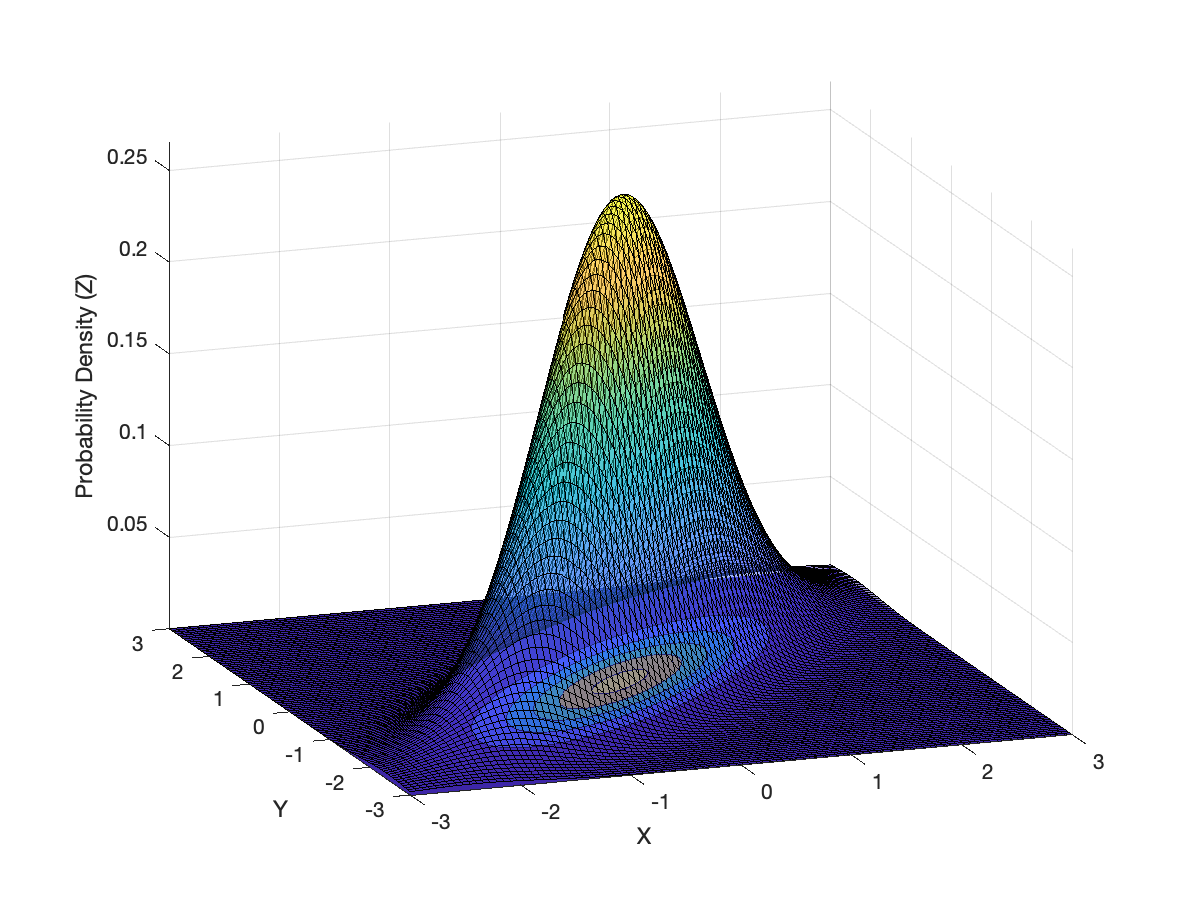
\includegraphics[width=0.75\textwidth]{Figures/Background2/GaussuanSurface_Corr_0.8.eps}
        \vspace{-10pt}
        \caption{Bivariate Gaussian distribution ($\rho=0.4$).}
    \end{figure}
        \column{0.5\textwidth}
            \begin{figure}
    \centering
    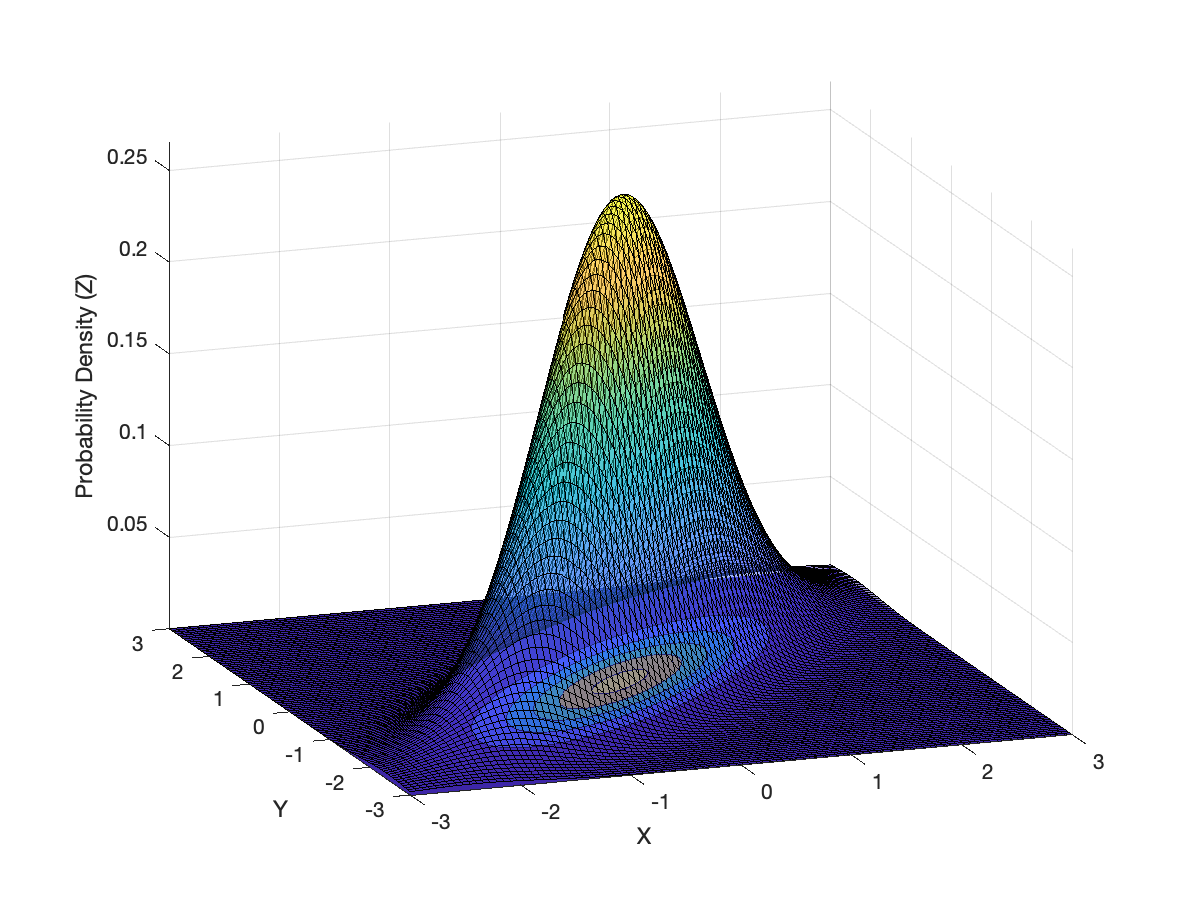
\includegraphics[width=0.75\textwidth]{Figures/Background2/GaussuanSurface_Corr_0.8.eps}
        \vspace{-10pt}
        \caption{Bivariate Gaussian distribution ($\rho=0.8$).}
    \end{figure}
\end{columns}



\end{frame}

%-------------------------------------------------------
\subsubsection{Bivariate Normal Distribution}
\begin{frame}{The Background Break - Bivariate Normal Distribution}
\begin{columns}
        \column{0.5\textwidth} 
For univariate distribution, the area between the $1\sigma$ boundaries is 68.26\% of the total area under the Gaussian function.
                \begin{figure}
            \centering
    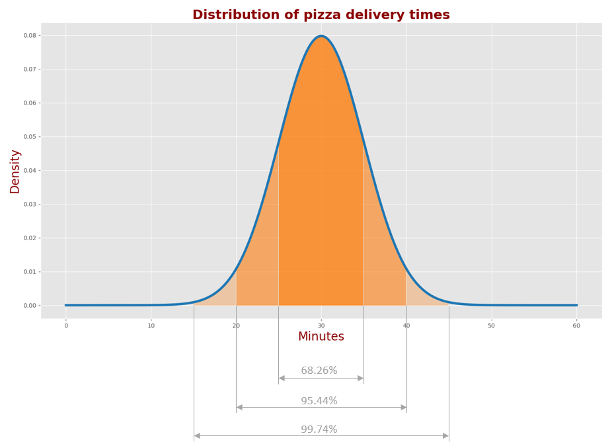
\includegraphics[width=1\textwidth]{Figures/Background2/UnivariateGaussian.png}
        \vspace{-10pt}
        \caption{Univariate Gaussian.}
    \end{figure}
        \column{0.5\textwidth}
        The probability of the bivariate normal distribution is a volume of the 3D
Gaussian function. For example, the volume of the 3D Gaussian function sliced at  $1\sigma$ 
level is 39.35\% of the total volume of the 3D Gaussian function.
        \begin{figure}
            \centering
    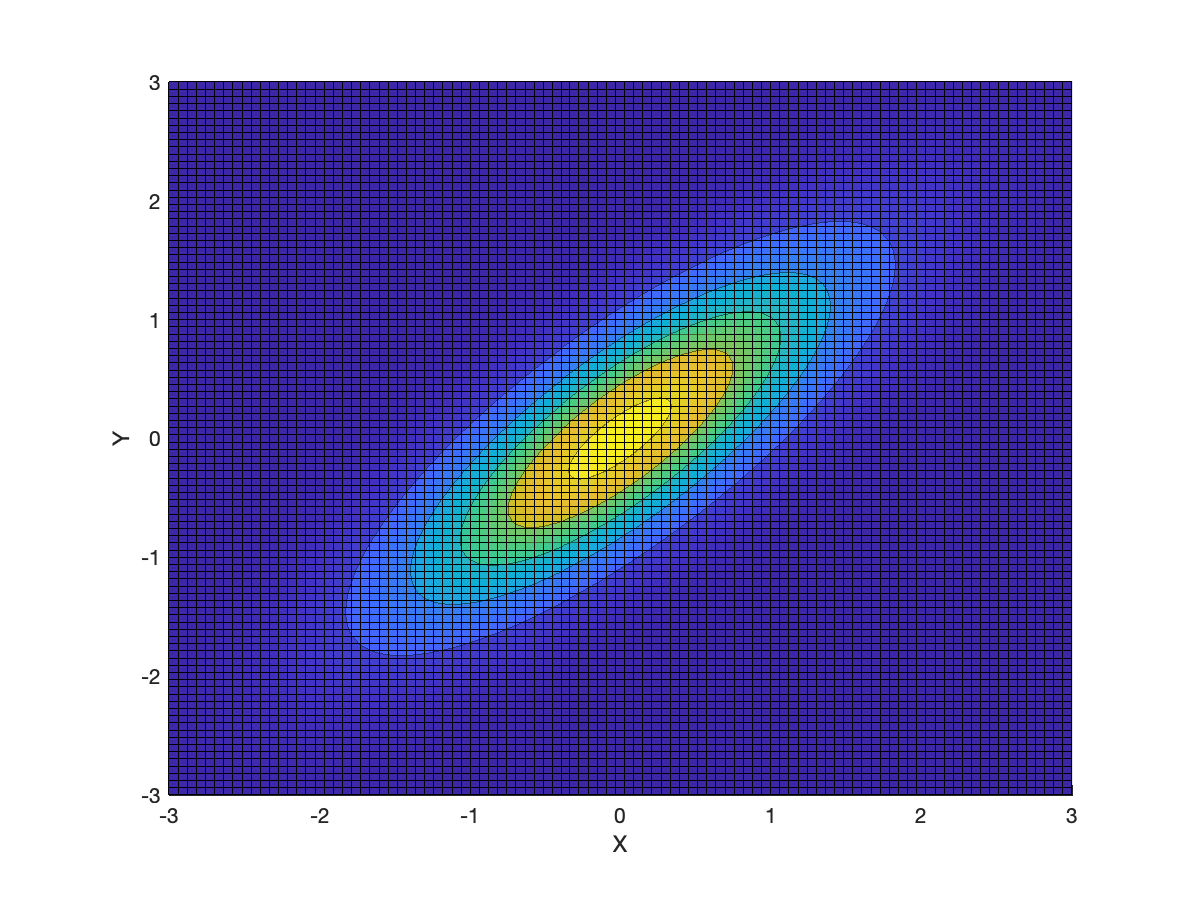
\includegraphics[width=1\textwidth]{Figures/Background2/GaussianContour_Corr_0.8.eps}
        \vspace{-10pt}
        \caption{Bivariate Gaussian distribution - Contour ($\rho=0.4$).}
    \end{figure}
    \texttt{\tiny [Code: Multivariate KF/bivariateGaussian\_withContours.m]}
\end{columns}
\end{frame}
%-------------------------------------------------------
\subsubsection{Covariance Ellipse}
\begin{frame}{The Background Break - Bivariate Normal Distribution - Covariance Ellipse}

\begin{itemize}
    \item The covariance ellipse represents an \textit{iso-contour} of the Gaussian distribution and allows visualization of a $1\sigma$ confidence interval in two dimensions. 
    \item It provides a geometric interpretation of the covariance matrix.
    \item Any ellipse can be described by four parameters:
    \begin{itemize}
        \item Ellipse center $\mu_x$, $\mu_y$
        \item Half-major axis $a$
        \item Half-minor axis $b$
        \item Orientation angle $\theta$
    \end{itemize}
    \begin{figure}
        \centering
        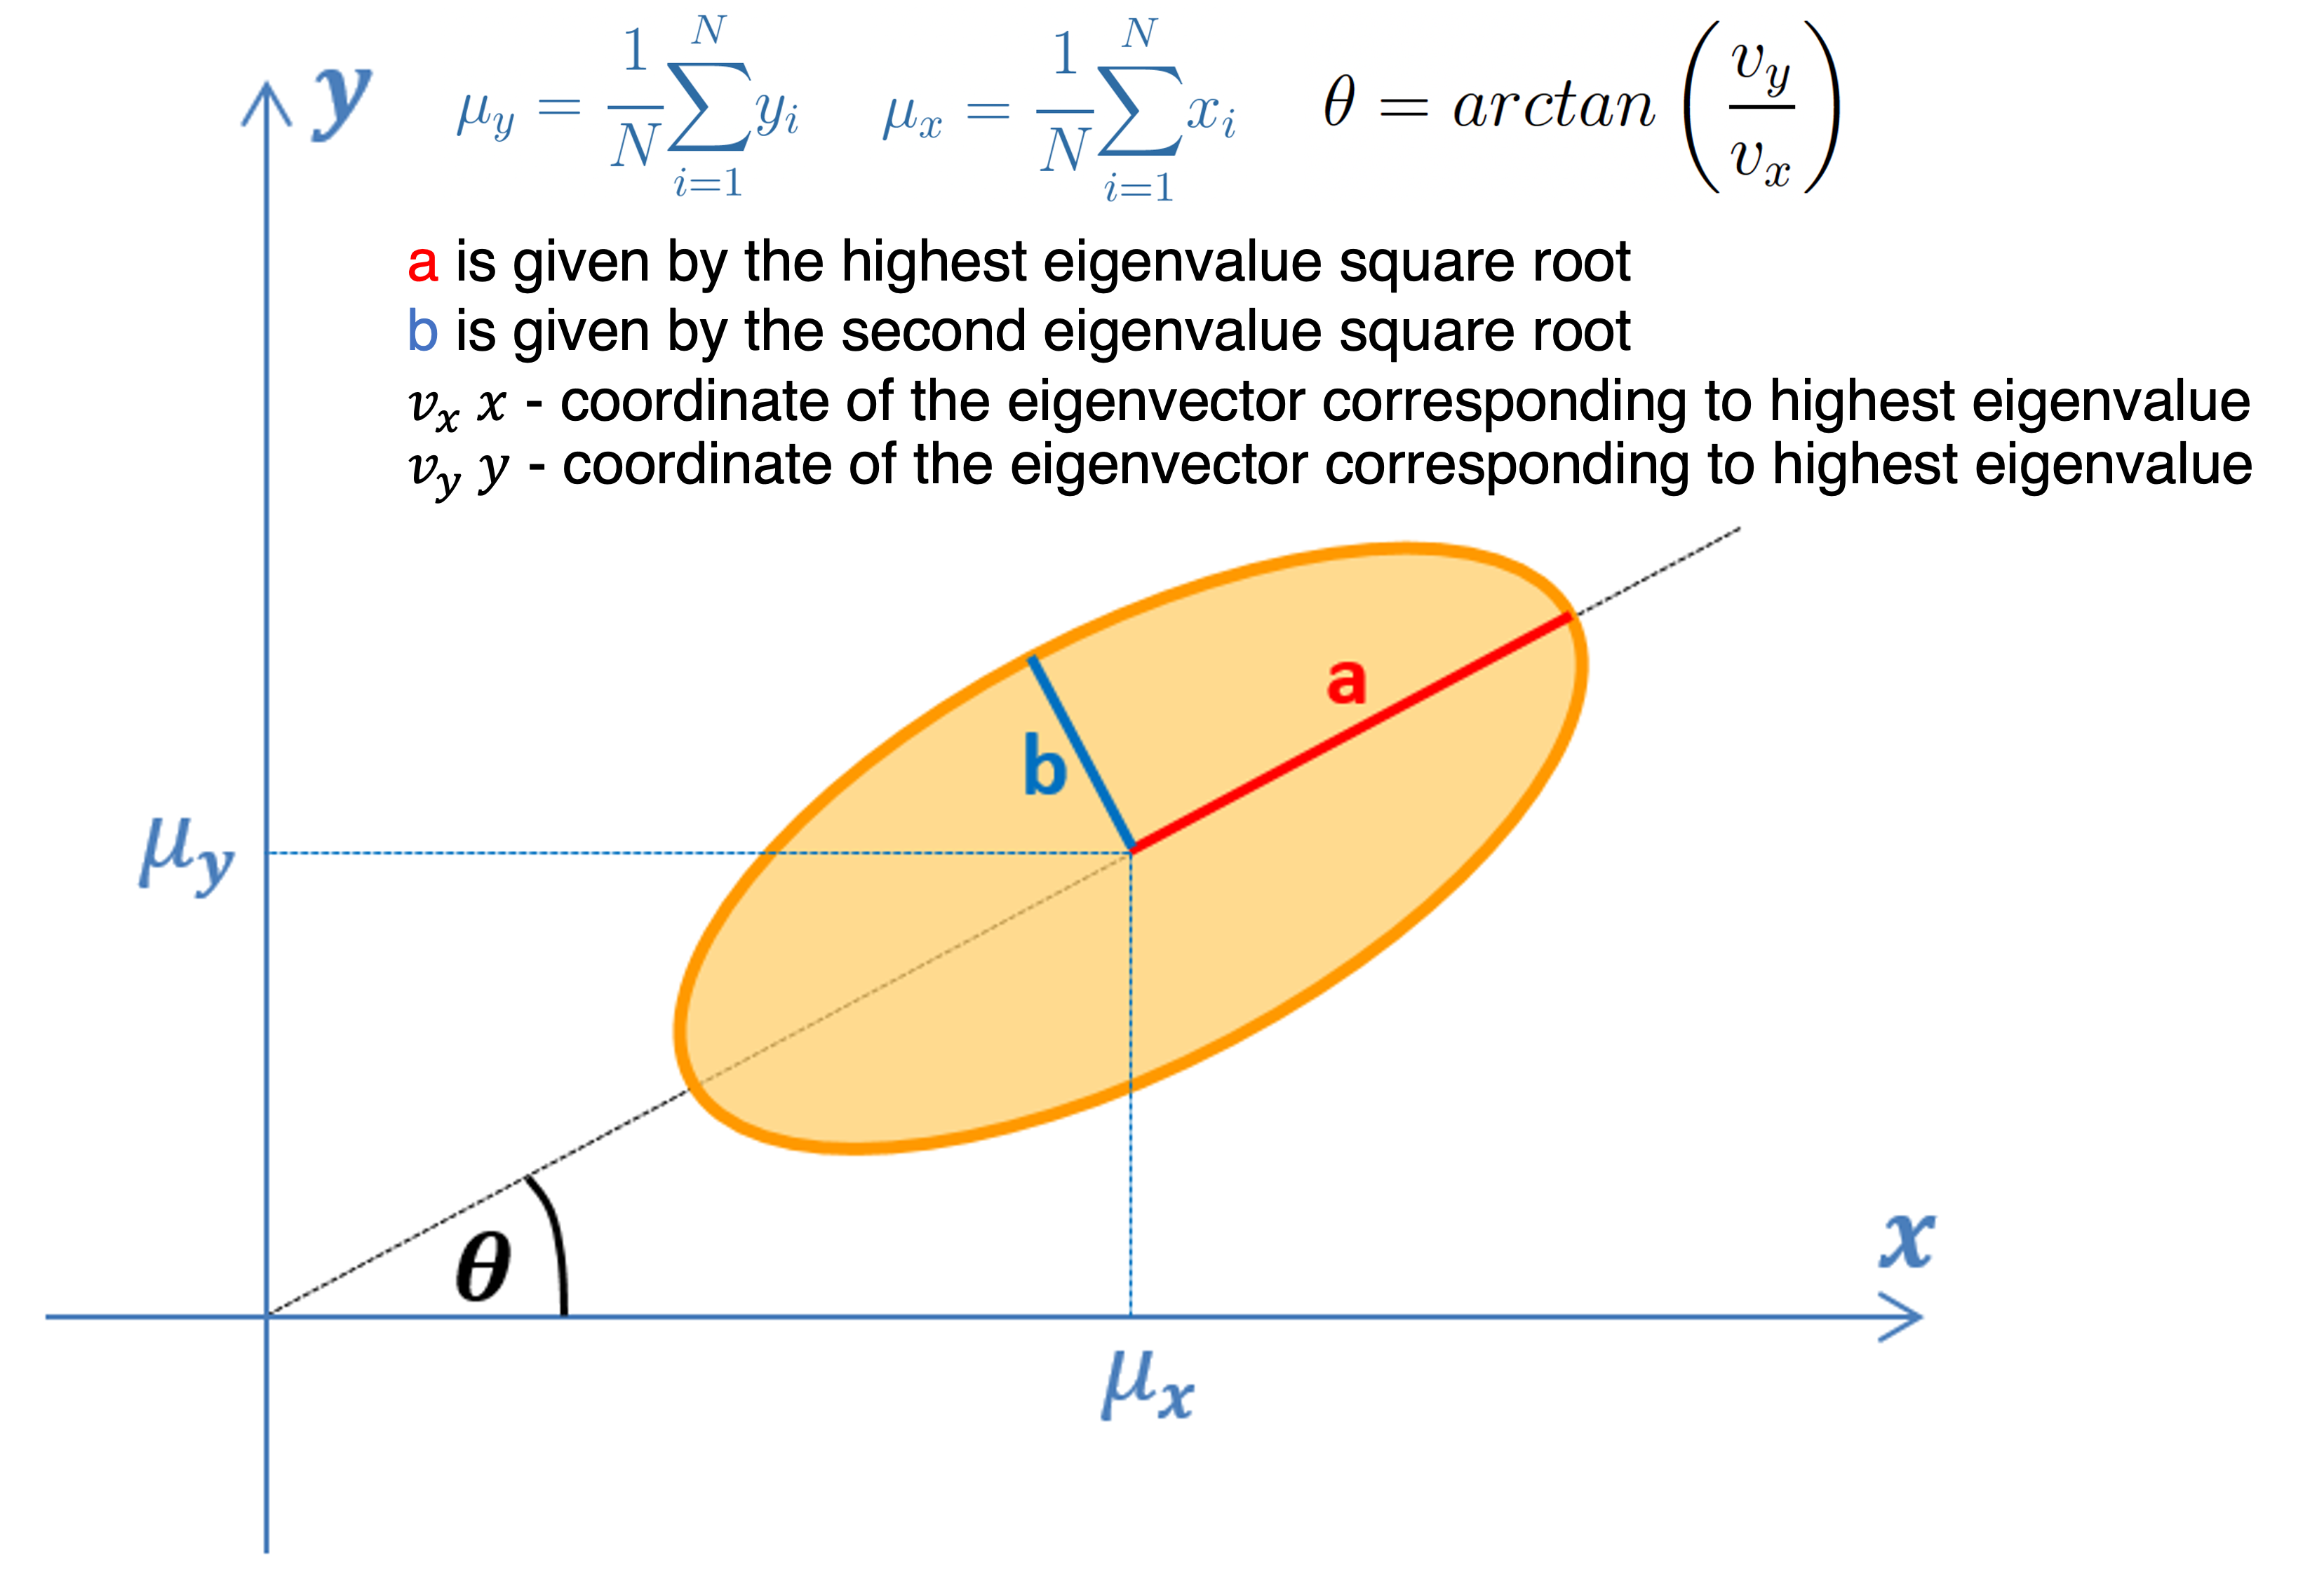
\includegraphics[width=0.6\textwidth]{Figures/Background2/CovarianceEllipse.png}
        \vspace{-10pt}
        \caption{Covariance ellipse.}
    \end{figure}
    

\end{itemize}

\end{frame}
%-------------------------------------------------------
\subsubsection{Confidence Ellipse}
\begin{frame}{The Background Break - Confidence Ellipse and Finding Probability Boundaries}

\begin{itemize}
    \item Often there is an interest in finding the boundaries of specific probability. For example, for 95\% probability, we should find the boundary that includes 95\% of Gaussian function volume.
    \item The projection of this boundary onto the \(x - y\) plane is the confidence ellipse. 
    \item \textbf{Find an elliptical scale factor \(k\), that extends the covariance ellipse to the confidence ellipse associated with 95\% probability.}
    \end{itemize}
    \begin{figure}
        \centering
        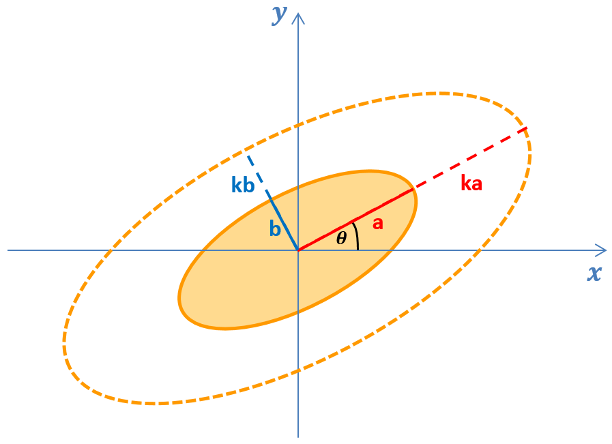
\includegraphics[width=0.6\textwidth]{Figures/Background2/ConfidenceEllipse.png}
        \vspace{-10pt}
        \caption{Covariance ellipse.}
    \end{figure}
\end{frame}
\begin{frame}{The Background Break - Confidence Ellipse and Finding Probability Boundaries}
   \begin{itemize} 
    \item As \(\sigma_x\) and \(\sigma_y\) represent the standard deviations of stochastically independent random variables, the addition theorem for the chi-square distribution may be used to show that the probability associated with a confidence ellipse is given by:
    $$p = 1 - \exp\left(-\frac{1}{2}k^2\right)$$
    \item For a covariance ellipse \(k = 1\), the probability associated with a covariance ellipse is:
    $$p = 1 - \exp\left(-\frac{1}{2}\right) = 39.35\%$$
    \item For a given probability, we can find an elliptical scale factor: $$k = \sqrt{-2\ln(1 - p)}$$
    \item For the probability of 95\%: $$k = \sqrt{-2\ln(1 - 0.95)} = 2.45$$
\end{itemize}

The properties of the confidence ellipse associated with 95\% probability are:
\begin{itemize}
    \item Ellipse center \((\mu_x, \mu_y)\) is similar to the covariance ellipse.
    \item Orientation angle \(\theta\) is similar to the covariance ellipse.
    \item Half-major axis length is \(2.45a\) – a scaled half-major axis of the covariance ellipse.
    \item Half-minor axis length is \(2.45b\) – a scaled half-minor axis of the covariance ellipse.
\end{itemize}
\end{frame}